\documentclass[border=10pt]{standalone}
\usepackage{pgfplots}
\pgfplotsset{width=7cm,compat=newest}


\begin{document}
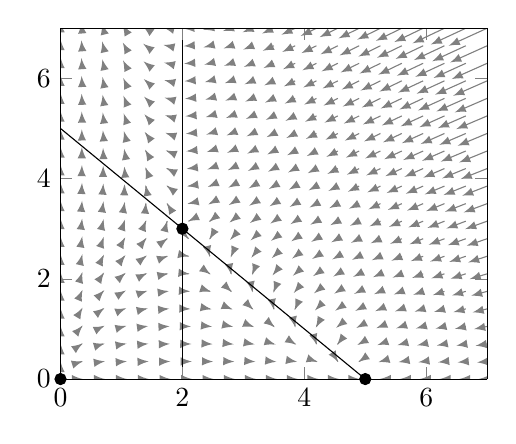
\begin{tikzpicture}
  \begin{axis}[
      view     = {0}{90},
      domain   = 0:7,
      y domain = 0:7,
      samples  = 21,
      xmin     = 0,
      xmax     = 7,
      ymin     = 0,
      ymax     = 7
    ]
    \addplot3 [
        gray,
        quiver={
            u={5*x-x^2-x*y},
            v={2*y-x*y},
            scale arrows=0.01,
            every arrow/.append style={-latex}
        }] (x,y,0);
    \addplot [mark=*] coordinates {(0,0)};
    \addplot [mark=*] coordinates {(2,3)};
    \addplot [mark=*] coordinates {(5,0)};
    \addplot [mark=*] coordinates {(2,-1) (2,8)};
    \addplot [mark=None] {-x+5};


  \end{axis}
\end{tikzpicture}
\end{document}
